\section{Medidas de tendencia central}
\subsection{Media aritmética}
La media aritmética de una población (datos) se representa por la letra $\mu$ (mu). La manera de calcularla es la siguiente:
Para datos:
\begin{equation}
    \mu = \sum_{i=1}^N \frac{x_i}{N}
\end{equation}

Para clases:
\begin{equation}
    \mu = \sum_{i=1}^k \frac{f_ix_i}{N} \qquad N=\sum_{i=1}^k f_i
    \label{eq:media_ponderada}
\end{equation}

donde $f_i$ es la frecuencia de cada clase.

\subsection{Media ponderada}
Su definición es la misma que la media para las clases (Eq. \ref{eq:media_ponderada}), en este caso $f_i$ es el peso del dato..

\subsection{Mediana}
La mediana de un conjunto de datos $\{\chi_i\}$ se define como el valor que se encuentra en medio cuando los datos son ordenados en orden creciente. Sea N el número total de datos, entonces, la mediana es:
\begin{equation}
    \text{Median} = \left\lbrace\begin{matrix}
        \chi_{int(\frac{N}{2})+1} \qquad \text{si} \qquad N\text{ es impar}                     \\
        \\
        \frac{\chi_{\frac{N}{2}}+\chi_{\frac{N}{2}}}{2} \qquad \text{si} \qquad N\text{ es par} \\
    \end{matrix} \right.
\end{equation}

Para clases, la mediana se obtiene de la siguiente manera:
\begin{equation}
    \text{Median}= L_1+\left(\frac{\frac{N}{2}-\sum f_i}{f_{Median}}\right)C
    \label{eq:median_class}
\end{equation}
donde: \begin{itemize}
    \item $L_i$: Es el límite inferior de la clase que contiene a la mediana.
    \item N: Es el número total de datos.
    \item $\sum f_i$: Es la suma de las frecuencias de las clases por debajo de la clase mediana.
    \item $f_{median}$: Es la frecuencia de la clase mediana.
    \item C: Tamaño del intervalo de la clase mediana (antes definido como $R_c$).
\end{itemize}

Por ejmeplo, tomando los datos de la tabla \ref{table:valores_aleatorios_introduccion} y los resultados de la tabla \ref{table:histograma_de_clases_introduccion}, se tiene que la mediana de los datos es 146. Por lo tanto $L_i=145.5$, esto es porque la clase que lo contiene es 146-154. El total de datos es $N=40$, por lo tanto $\frac{N}{2}=20$, calculando la suma de las frecuencias se obtiene lo siguiente:
\begin{align*}
    \sum f_i & = f_1 + f_2 +f_3+f_4 \\
             & = 3 + 6 + 10         \\
             & =19
\end{align*}
de la tabla \ref{table:histograma_de_clases_introduccion} se obtiene que $f_{Median}=11$, y de los calculos realizados en la ecuación \ref{eq:r_c} se tiene que $C=9$. Por lo tanto realizando los calculos definidos en la ecuación \ref{eq:median_class} se tiene  que la mediana de estos datos agrupados por clases es igual a 146.3.

\section{Moda}
La moda de un conjunto de números es el valor que se presenta con mayor frecuencia. La moda puede no existir y no necesariamente es única. La moda para las clases esta definida de la siguiente manera:
\begin{equation}
    \text{Moda}= L_i+ \left(\frac{\Delta f_{i,i-1}}{\Delta f_{i,i-1}+\Delta f_{i,i+1}}\right)C
    \label{eq:moda}
\end{equation}
donde\begin{itemize}
    \item $L_i$: Es el límite inferior de la clase que contiene mayor frecuencia.
    \item $\Delta f_{i,i-1}$: Es la diferencia de frecuencias de la clase modal y la anterior.
    \item $\Delta f_{i,i+1}$: Es la diferencia de frecuencias de la clase modal y la siguiente.
    \item C: Tamaño del intervalo de la clase mediana (antes definido como $R_c$).
\end{itemize}
Usando como ejemplo los datos contenidos en la tabla \ref{table:valores_aleatorios_introduccion} y \ref{table:histograma_de_clases_introduccion}, se tiene que la clase modal es 146-154, ya que esta contiene una mayor cantidad de datos. Por lo tanto $L_i=145.5$. Calculando las diferencias entre frecuencias se tiene que:\\
\begin{minipage}{0.5\linewidth}
    \begin{align*}
        \Delta f_{i,i-1} & = 11-10 \\
                         & =1
    \end{align*}
\end{minipage}
\begin{minipage}{0.5\linewidth}
    \begin{align*}
        \Delta f_{i,i+1} & =11-5 \\
                         & =6
    \end{align*}
\end{minipage}
Entonces, usando la ecuación \ref{eq:moda} se tiene que la moda para estos datos es 146.78.
\subsection{Media geometrica}
\begin{equation*}
    MG=\sqrt[N]{\bigcup_{i=1}^N \chi_i}
\end{equation*}
\subsection{Media armonica}
\begin{equation*}
    \frac{1}{MA} = \sum_{i=1}^N \frac{1}{\chi_i N}
\end{equation*}
\subsection{Media cuadratica}
\begin{equation*}
    MQ= \sqrt{\sum_{i=1}^N \frac{\chi_i^2}{N}}
\end{equation*}
\section{Tipo se curvas de frecuencia}
\begin{figure}[H]
    \centering
    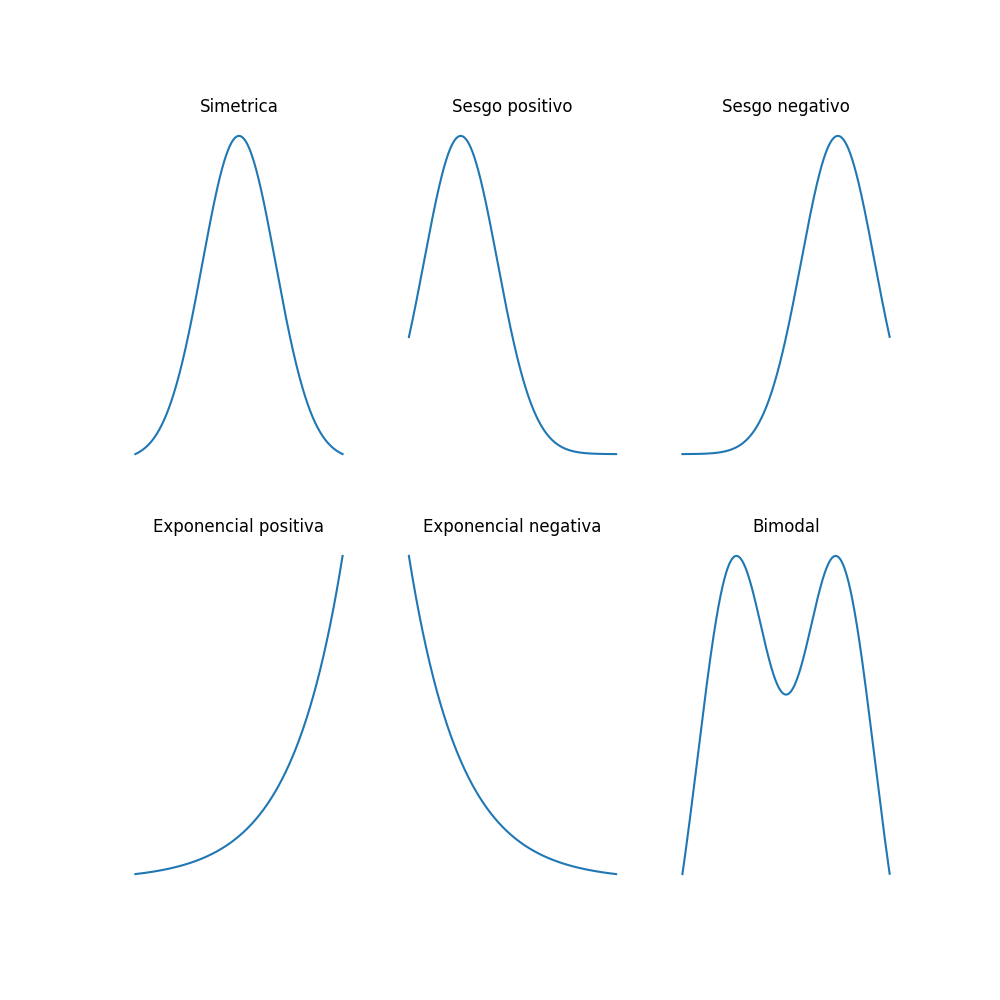
\includegraphics[scale=0.55]{Graphics/Frecuency_types.png}
\end{figure}
\section{Medidas de dispersión}
\subsection{Rango}
El rango es la diferncia entre el el valor mayor y el valor menor.
\subsection{Desviación media absoluta}
\begin{equation*}
    DAM= \sum_{i=1}^N \frac{|\chi_i-\mu|}{N}
\end{equation*}
donde $\mu$ es la media aritmética.
\subsection{Varianza y desviación estandar}
La definición de la varianza esta muy relacionada a la desviación estandar, las cuales son las siguientes respectivamente:
\begin{equation*}
    \sigma^2 = \sum_{i=1}^N \frac{(\chi_i-\mu)^2}{N} \qquad \sigma^2\rightarrow\text{varianza}
\end{equation*}
\begin{equation*}
    \sigma = \sqrt{\sum_{i=1}^N \frac{(\chi_i-\mu)^2}{N}} \qquad \sigma\rightarrow\text{desviacion estandar}
\end{equation*}
Para clases se tiene que:
\begin{equation*}
    \sigma^2 = \sum_{i=1}^N \frac{f_i(\chi_i-\mu)^2}{N}
\end{equation*}
\begin{equation*}
    \sigma = \sqrt{\sum_{i=1}^N \frac{f_i(\chi_i-\mu)^2}{N}}
\end{equation*}
Para muestras se tiene que $N=n-1$